\section{Boundary and exact-SGD experimental protocols}\label{app:extension_experiments}
All extension grids are specified in \texttt{experiments/extend.py}. Scientific tables are deterministic; runtime and machine metadata are recorded separately. No row is dropped based on whether a candidate helps. The mathematical claims assume exact arithmetic. Float64 audits use explicit tolerances, while separate mpmath checks use 80 digits. A passed test is not a proof of an inequality outside its tested inputs.

\subsection{Arbitrary schedules and the local boundary}
The arbitrary-schedule audit draws 1,200 cases with seed 921004. Angles are uniform on $[0.15,1.45]$ radians; budgets are log-uniform on $[0.1,15]$; orthogonal masses are the exact boundary times a log-uniform factor on $[0.03,5]$. Ridges are sampled from $\{0,0.02,0.1\}$, and phase counts from $\{1,2,3,8,16,64\}$. Durations are Dirichlet proportions of the budget. Half the paths use pure sources; the others use uniform mixture weights. The table records the transition risk, slow-column length, and separate lower bounds. There are no observed violations at the declared tolerance of order $10^{-11}$.

The independent high-precision audit uses angles $15,30,45,65,80$ degrees; budgets $0.1,0.5,1,4,8$; and boundary multipliers $0.1,0.5,0.99,1,1.01,2$. It evaluates two $2\times2$ exponentials directly at 80 decimal digits with perturbation amplitude $10^{-5}\sqrt{ad}$. All 150 relative improvements have the predicted sign. At the boundary itself, the finite perturbation is not claimed to tie the optimum; it cannot improve it.

The near-boundary audit uses angles $30,45,65$ degrees, budgets $1,4,8$, and $\xi\in\{10^{-2},10^{-3},10^{-4},10^{-5},10^{-6}\}$. The coefficient $K$ is computed by high-precision quadrature of the explicit first variation in Appendix~\ref{app:global}, split at the switch. All 45 perturbations are feasible. We record the witness coefficient, the global upper coefficient, and the theoretical limit separately. At $\xi=10^{-6}$ the witness coefficient is within $2\times10^{-5}$ of $1/8$ in all nine geometry--budget pairs. Figure~\ref{fig:near} shows the $B=4$ cases.

\begin{figure}[h]
\centering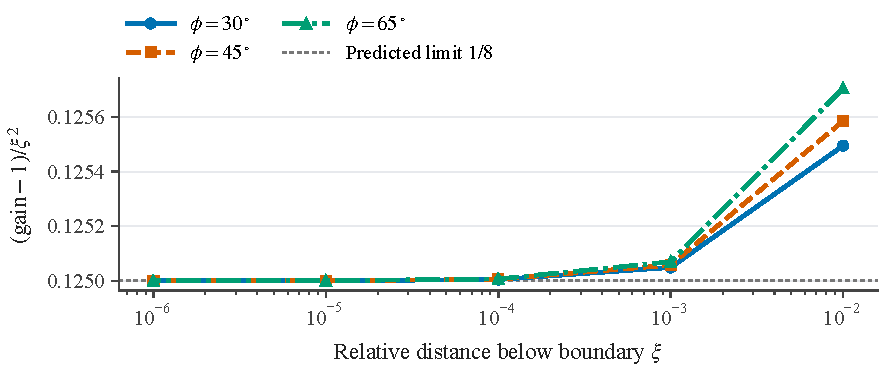
\includegraphics[width=.92\linewidth]{figures/boundary_coefficient.pdf}
\caption{The attainable two-phase gain approaches the sharp all-schedule coefficient $1/8$ near the boundary. Each curve fixes the angle and $B=4$, then varies the relative boundary distance. Values use 80-digit exponentials, not a fit to float64 cancellation.}\label{fig:near}
\end{figure}

The boundary curves in the main text use angles $30,45,65$ degrees; masses $0,10^{-4},10^{-3},10^{-2},0.1$; ridge $0.02$; and 100 budgets from $0.2$ to 12. Candidates include static mixing, the pure preparation rule when feasible, and a bounded scalar search over the mixed witness amplitude. These are attainable lower bounds on the optimal gain. No global optimizer is claimed below the exact boundary.

\subsection{Additive-noise checks}
For 480 cases with seed 921005, angles are uniform on $[0.2,1.4]$, budgets on $[0.1,20]$, masses in $\{0,0.001,0.1,1\}$, noise amplitudes in $\{0.01,0.1,0.3\}$, and phase counts in $\{1,2,5,20\}$. Ridge is 0.02. Each phase is solved through its symmetric eigendecomposition and the exact Ornstein--Uhlenbeck covariance integral. We record deterministic-plus-noise risk, the isolated noise contribution, and both theoretical lower bounds. No violations are observed. Separate curves fix $45^\circ$, zero orthogonal mass, ridge 0.02, and 121 budgets from 1 to 24 for $\sigma\in\{0,0.001,0.01,0.1\}$. The zero-noise gain ceiling is finite because it includes the energy lower bound, not only the vanishing determinant bound.

\begin{figure}[h]
\centering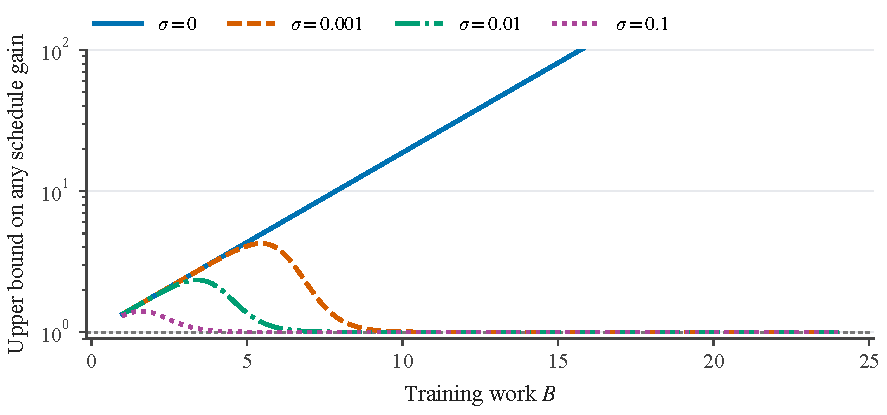
\includegraphics[width=.92\linewidth]{figures/diffusion_ceiling.pdf}
\caption{A global upper bound on the gain of any deterministic schedule in the stated additive-noise model. Positive isotropic noise eventually drives the ceiling to one. These are bounds, not achieved gains and not an SGD diffusion fit.}\label{fig:diffusion}
\end{figure}

\subsection{Exact expected Gaussian SGD}
The full grid has angles $30,45,65$ degrees, work $B\in\{1,4,8\}$, steps $\eta\in\{0.01,0.05\}$, batch sizes $m\in\{1,8,64\}$, label standard deviations $\sigma_y\in\{0,0.1\}$, and orthogonal masses $\varepsilon\in\{0,10^{-4},0.01,0.1\}$. Source covariance is \eqref{eq:mainfamily} with ridge 0.02. There are $K=B/\eta$ updates and $Km$ examples per comparison. We repeat the same 432 conditions for per-example and per-batch source selection. This yields 864 deterministic moment calculations; there is no finite-trial sampling error in their expected risks.

For each condition, the static comparator is the global lower/upper bracket of Appendix~\ref{app:moments}. Every recorded relative width is below $10^{-3}$. The schedule library consists of every integer pure-source switch in both orders, mixed witnesses with amplitude fractions $0.01,0.05,0.1,0.25,0.5,0.75,1$, and the best static grid point. Mixed witnesses split the updates as $\lfloor K/2\rfloor$ and $K-\lfloor K/2\rfloor$. Pure-switch risks are evaluated by composing exact moment operators, not by fitting an exponential. The flow-rule switch $\tau$ is rounded to the nearest update; it is reported separately when feasible (384 of 432 settings for each sampling convention).

Descriptive candidate and flow-rule gains use the best evaluated static risk (the upper bracket) in the numerator; gain counts use the lower bracket. The lower-bracket gain exceeding 1.01 occurs in 186 per-example and 220 per-batch settings. Their maximal candidate gains are 2.5855 and 8.9237, respectively; these maxima are descriptive and are not the headline evidence. Median gains and the full grid show the limited and noise-dependent nature of the improvements. The 18 aggregated conditions below include both successful and unsuccessful settings. The candidate library includes static mixing, so a median of one is a tie by construction, not evidence that every proposed curriculum is safe.
\begin{table}[h]\centering\small
\caption{Complete aggregated Gaussian SGD conditions. Each row includes 48 settings. Median gains use the upper static bracket; $>1\%$ counts use the lower bracket.}
\begin{tabular}{llrrrr}\toprule Sampling & Batch & $B$ & Median candidate & Median flow rule & $>1\%$ gains\\\midrule
batch & 1 & 1 & 1.0189 & 0.8783 & 42 \\
batch & 1 & 4 & 1.0000 & 0.7790 & 6 \\
batch & 1 & 8 & 1.0000 & 0.1932 & 0 \\
batch & 8 & 1 & 1.0209 & 0.8702 & 44 \\
batch & 8 & 4 & 1.3605 & 1.3574 & 28 \\
batch & 8 & 8 & 1.0000 & 0.3705 & 8 \\
batch & 64 & 1 & 1.0214 & 0.8698 & 44 \\
batch & 64 & 4 & 1.5414 & 1.5361 & 28 \\
batch & 64 & 8 & 1.0000 & 0.6407 & 20 \\
example & 1 & 1 & 1.0189 & 0.8783 & 42 \\
example & 1 & 4 & 1.0000 & 0.7790 & 6 \\
example & 1 & 8 & 1.0000 & 0.1932 & 0 \\
example & 8 & 1 & 1.0171 & 0.8688 & 40 \\
example & 8 & 4 & 1.0269 & 0.9891 & 25 \\
example & 8 & 8 & 1.0000 & 0.1787 & 0 \\
example & 64 & 1 & 1.0169 & 0.8682 & 40 \\
example & 64 & 4 & 1.1633 & 1.1627 & 28 \\
example & 64 & 8 & 1.0000 & 0.1844 & 5 \\
\bottomrule\end{tabular}\end{table}


\paragraph{Independent Monte Carlo validation.}
We fix $45^\circ$, ridge 0.02, $\varepsilon=0.001$, $\eta=0.05$, $B\in\{2,4\}$, $m\in\{1,8\}$, and $\sigma_y\in\{0,0.1\}$. Both sampling conventions are tested, with static and selected two-phase methods, yielding 32 conditions. Each uses 8,192 independent trajectories. Initial errors are $u\pm\sqrt\varepsilon v$ with equiprobable signs, so their second moment is exactly the theoretical input in expectation. Fresh Gaussian examples and independent noise are drawn at every update. Within each condition methods share a seed for paired comparisons, but trajectories are independent across the 8,192 replicates. Standard errors use the sample standard deviation of terminal losses divided by the square root of this replicate count. All 32 means lie within three standard errors of the exact risk; the largest absolute standardized discrepancy is 2.096. This is a model-implementation check, not a familywise statistical claim.

\paragraph{Oracle versus paid computation.}
The moment library assumes that the source covariances, label variance, and initial second moment are known. Search cost is not included in its work axis. It therefore measures whether a schedule helps the training dynamics under equal update/example counts. It does not establish a practical cost saving after estimating these moments. The separate paid-pilot experiment explicitly accounts for its own observation and declared planning costs, and retains its poor all-outcome performance.
